\section{Implementierung}
\label{sec:implementierung}

In diesem Abschnitt wird die Implementierung des in Abschnitt \ref{sec:konzept} vorgestellten Konzepts erläutert. Dazu werden als zunächst die Voraussetzungen für das Ausführen der Anwendung und die Einrichtung der Server beschrieben (siehe Abschnitt \ref{sec:voraussetzungen}). Anschließend wird das entwickelte Skript vorgestellt (siehe Abschnitt \ref{sec:setupskript}) und die dazu gehörige Konfigurationsdatei erläutert (siehe Abschnitt \ref{sec:konfigurationsdatei}). Zum Abschluss wird der Ablauf des Skripts erläutert (siehe Abschnitt \ref{sec:ablauf}).

\subsection{Voraussetzungen}
\label{sec:voraussetzungen}

Für die Bereitstellung einer Wikipedia-Instanz benötigt ein Server folgende Software:
\begin{itemize}
\item Webserver (empfohlen Apache \texttt{httpd})
\item PHP (empfohlen $\geq$ 5.0)
\item MySQL (empfohlen $\geq$ 4.0)
\item ImageMagick (empfohlen zur Generierung von Thumbnails)
\end{itemize}

Außerdem wird auf dem Rechner, auf dem das Setup-Skript ausgeführt wird, mindestens Python 2.6 benötigt und gegebenenfalls \texttt{gnuplot}. Zudem muss ein Mediawiki installiert und der Wikipedia-Dump in die Datenbank eingespielt sein. Auf den Servern, auf denen die Wikipedia-Umgebung installiert wird, ist mindestens Python 2.4 erforderlich.

In der konkreten Umsetzung wird die Mediawiki Version 1.16.5 genutzt und der Dump der Wikipedia Artikel zuerst mit dem Programm \texttt{xml2sql}\footnote{\url{http://meta.wikimedia.org/wiki/Xml2sql/}} in SQL transformiert und dann mit dem Programm \texttt{mysqlimport} in die Datenbank importiert. Dieses Verfahren wird offiziell nicht empfohlen, aber es stellte sich als schneller und sicherer heraus als die Nutzung des PHP-Skripts vom Mediawiki.

Anschließend muss die Datenbank in diesem Zustand gesichert werden, da dieser Stand der Datenbank wieder benötigt wird, falls ein anderer Abschnitt des Traces vorbereitet werden soll. Dazu ist das MySQL-Verzeichnis (z.B. \texttt{/var/lib/mysql/}) per \texttt{tar} zu packen und gegebenenfalls noch per \texttt{gzip} oder \texttt{bzip2} komprimiert werden. Das Archiv darf keine absoluten Pfade enthalten und muss von der Wurzel des MySQL-Verzeichnisses erstellt werden. Dieses Archiv wird später bei der Konfiguration des Setup-Skripts benötigt.

Nach der Installation vom Mediawiki (der Ordner des Mediawikis muss \glqq{}w/\grqq{} genannt werden) muss die Datei \texttt{LocalSettings.php} noch angepasst werden. Dazu müssen folgende Zeilen ergänzt werden:
\begin{verbatim}
$wgArticlePath      = '/wiki/$1';
$wgScriptPath       = "/w";

$wgMaxShellMemory   = "unlimited";
$wgMaxShellFileSize = "unlimited";

require_once( "$IP/extensions/Cite/Cite.php" );
require_once( "$IP/extensions/ImageMap/ImageMap.php" );
require_once( "$IP/extensions/OggHandler/OggHandler.php" );
require_once( "$IP/extensions/ParserFunctions/ParserFunctions.php" );
\end{verbatim}
Die angegebenen Extensions müssen dann noch heruntergeladen werden und in dem Ordner \texttt{extensions} hinterlegt werden. Dies ist z.B. über das SVN-Repository\footnote{\url{http://svn.wikimedia.org/svnroot/mediawiki/tags/REL1_16_5/extensions/}} des Mediwiki möglich. Damit der Apache httpd Server mit den verschiedenen URL-Formen der Wikipedia zurecht kommt, muss noch folgender Eintrag in der httpd-Konfigurationsdatei (welche z.B. unter  \texttt{/etc/httpd/conf/httpd.conf} zu finden ist) ergänzt werden (wobei der Pfad zur \texttt{index.php} anzupassen ist):
\begin{verbatim}
Alias /wiki "/var/www/html/w/index.php"
\end{verbatim}
Es gibt noch weitere Möglichkeiten die Unterstützung der Short-URLs von Wikipedia zu erreichen, diese sind in dem Mediawiki Wiki\footnote{\url{http://www.mediawiki.org/wiki/Manual:Short_URL}} nachzulesen.

Bei der Verwendung von Red-Hat basierten Systemen (wie z.B. CentOS) ist zu beachten, dass in dem Paket \texttt{gnome-vfs2} bis zur Version 2.16.2-8.el5 ein Bug\footnote{\url{http://rhn.redhat.com/errata/RHBA-2011-0441.html}} die korrekte Ausführung von ImageMagick verhindert. Dadurch können keine Thumbnails für SVG-Dateien erstellt werden. Daher ist es empfehlenswert, mindestens die genannte Version des Pakets zu installieren.

\subsection{Setup-Skript}
\label{sec:setupskript}
Die entwickelte Anwendung ist ein Python 2.6 Skript \texttt{setup\_env.py} und nutzt das ebenfalls selbst entwickelte Modul \texttt{ppr}. Der Sourcecode liegt der Ausarbeitung bei oder kann aus einem GIT-Repository\footnote{\url{https://github.com/menski/ppr-s11}} heruntergeladen werden.

In Abbildung \ref{fig:classes} wird das Klassendiagramm des \texttt{ppr} Moduls gezeigt. Die Basis-Klasse \texttt{Process} erbt von der Klasse \texttt{multiprocessing.Process}. Daran ist zu erkennen, dass fast jede Klasse ebenfalls ein eigener Prozess ist. Somit können verschiedene Aufgaben in dem Skript parallel durchgeführt werden. Die Kommunikation zwischen den Prozessen wird über sogenannte \texttt{Pipes} realisiert, wodurch Daten nicht lange im Speicher gehalten werden müssen.

\begin{figure}
  \centering
  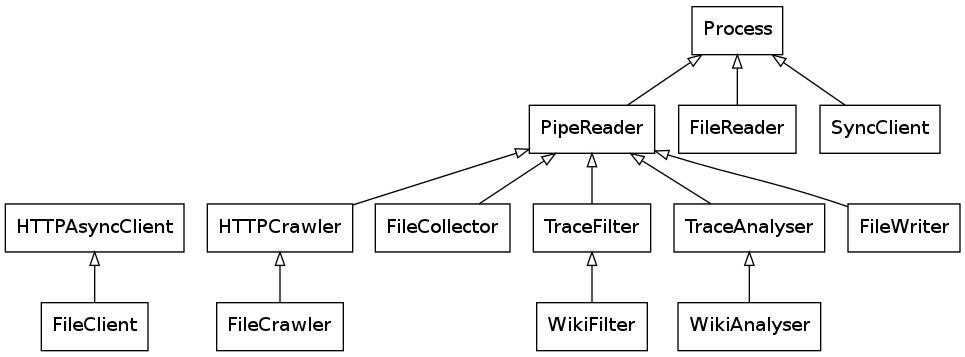
\includegraphics[width=\textwidth]{images/classes.png}
  \caption{Klassendiagramm des \texttt{ppr}-Moduls}
  \label{fig:classes}
\end{figure}

\subsubsection{Klassenübersicht}
\label{sec:klassen}

Das entwickelte Skript gliedert sich in folgende Klassen:

\begin{description}
\item[Process:] Basis-Klasse, welche von \texttt{multiprocessing.Process} erbt und einen Logger bereitstellt.
\item[SyncClient:] Ist eine Klasse, die genutzt wird, um eine Wikipedia-Instanz auf einen anderen Rechner zu kopieren.
\item[FileReader:] Diese Klasse liest eine Datei ein und sendet den Inhalt zur Verarbeitung an eine Menge von \texttt{Pipes}. Dabei ist es möglich, die Funktion zum Öffnen der Datei anzugeben, um z.B. komprimierte Dateien zu öffnen.
\item[PipeReader:] Eine Klasse, welche eine \texttt{Pipe} nach Außen anbietet, über die sie mit Daten versorgt werden kann.
\item[FileWriter:] Erbt von der Klasse \texttt{PipeReader} und speichert die übergebenen Daten in einer Datei. Wiederum ist es möglich, eine Funktion zum Öffnen der Datei anzugeben, um z.B. komprimierten Dateien zu schreiben.
\item[TraceAnalyser/WikiAnalyser:] Spezielle \texttt{PipeReader}, welche zur Analyse von Traces und zum Erstellen von Statistiken und Grafiken dienen.
\item[TraceFilter/WikiFilter:] Klassen zum Filtern von Traces, welche ebenfalls von \texttt{PipeReader} erben.
\item[HTTPAsyncClient/FileClient:] Klassen, welche das Python Modul \texttt{asynchat} nutzen um HTTP1.1 Requests zu versenden. Die Klasse \texttt{FileClient} kann außerdem den Response in einer Datei speichern.
\item[HTTPCrawler/FileCrawler:] Klassen, die unter Nutzung der Klassen \texttt{HTTPAsyncClient}/ \texttt{FileClient} und dem Python-Modul \texttt{asyncore}, asynchrone HTTP-Requests versendet.
\item[FileCollector:] Eine Unterklasse von \texttt{PipeReader}, welche überprüft ob eine Datei bereits im Dateisystem existiert und falls nicht, diese mit Hilfe der \texttt{FileCrawler} Klasse versucht herunterzuladen.
\end{description}

\subsubsection{Konfigurationsdatei}
\label{sec:konfigurationsdatei}

Ein vollständige Konfigurationsdatei ist im Anhang \ref{sec:konfiguration} aufgeführt. In diesem Abschnitt werden die einzelnen Bereiche der Konfigurationsdatei erläutert werden.

\paragraph{[general]}

In dem \texttt{general}-Abschnitt können die einzelnen Schritte des Skripts aktiviert bzw. deaktiviert werden (siehe dazu Abschnitt \ref{sec:konzept}). Außerdem kann das Log-Level gewählt und festgelegt werden, ob die Analyse eine Grafik, für die Requests pro Sekunde, mit \texttt{gnuplot} erstellt.

\paragraph{[trace]}

Der folgende \texttt{trace}-Abschnitt gibt den Pfad zur Trace-Datei an und ob sie mit \texttt{gzip} komprimiert ist.

\paragraph{[filter]}

Im \texttt{filter}-Abschnitt wird das Zeitintervall definiert, nachdem der Trace gefiltert wird. Dabei wird das Format $a:b$ genutzt und auf die folgende Weise interpretiert: $a$ ist ein UNIX-Zeitstempel, wenn $a > b$ gilt wird $b$ als Anzahl von Sekunden interpretiert und auf $a$ addiert, sonst wird $b$ ebenfalls als UNIX-Zeitstempel interpretiert. Als nächstes wird ein Hostname bestimmt, der genutzt wird um einen modifizierten Trace zu erstellen, welcher später zum Wiedereinspielen genutzt werden kann. Um nach bestimmten URLs zu filtern, kann ein regulärer Ausdruck angegeben werden. Abschließend kann festgelegt werden, ob die gefilterten Traces mit \texttt{gzip} komprimiert gespeichert werden.

\paragraph{[download]}

Der \texttt{download}-Abschnitt definiert das Verhalten beim Herunterladen von Bildern. Dazu wird ein Pfad angegeben, an dem nach bereits heruntergeladen Bilder gesucht wird und ebenfalls die neu heruntergeladenen Bilder gespeichert werden. Weiterhin kann der Port angegeben werden, über den die Requests versendet werden, um neue Bilder herunterzuladen. Die \texttt{async}-Option gibt die parallel aufgebauten, asynchronen Verbindungen an. Des Weiteren, werden die Pfade zu der Mediawiki- und MySQL-Installation, sowie der Name des lokal laufenden MySQL-Services benötigt. Mit den Optionen \texttt{clean\_images} und \texttt{clean\_mysql} kann bestimmt werden, ob die aktuell in der Mediawiki-Installation vorhanden Bilder anfangs gelöscht werden sollen, bzw. ob die Datenbank vor dem Einlesen der Bilder gelöscht werden soll und durch eine \glqq{}saubere\grqq{} Datenbank ersetzt werden soll. Diese \glqq{}saubere\grqq{} Datenbank wird über die Option \texttt{mysql\_archive} bestimmt. Die nach dem erfolgreichen Einrichten gepackten Mediawiki- und MySQL-Archive werden an dem Pfad gespeichert, der mit der Option \texttt{output\_dir} bestimmt wird.

\paragraph{[install]}

Der \texttt{install}-Abschnitt ist der letzte vorgegebene Abschnitt. Er besteht allein aus einem String, welcher die Server angibt auf denen die Wikipedia-Instanz installiert werden soll und die dafür vorgesehene Konfiguration. Dabei ist der String eine durch \glqq{}:\grqq{} getrennte Liste. Jedes Element besteht aus einem Konfigurationsnamen, welcher durch ein \glqq{}@\grqq{} von einer einer Liste (getrennt durch Kommata) von IP-Adressen oder Hostname getrennt ist. Für jeden angegebenen Konfigurationsnamen muss wiederum ein Abschnitt in der Konfigurationsdatei angelegt werden. 
In diesem Abschnitt wird der Name des Users und des MySQL-Services auf dem Server angegeben. Außerdem die Verzeichnisse in denen die übertragenen Daten gespeichert werden, das Mediawiki und die MySQL-Datenbank installiert sind.

\subsubsection{Ablauf}
\label{sec:ablauf}
In diesem Abschnitt wird der Ablauf des Skripts dargestellt und beschrieben, welche Dateien erstellt werden.

\begin{enumerate}
\item Die Konfigurationsdatei wird eingelesen und auf Korrektheit geprüft.
\item Sofern der Analyse-Schritt oder Filter-Schritt aktiviert wurde, wird ein \texttt{FileReader} für den Trace erzeugt. Ist eine Analyse gefordert wird ein \texttt{WikiAnalyser} erzeugt bzw. ist die Filterung gefordert ein \texttt{WikiFilter}. Der \texttt{FileReader} sendet nun die gelesen Daten an die erzeugten Instanzen. Wurde eine \texttt{WikiAnalyser}-Instanz erzeugt, erstellt diese für eine Trace-Datei \texttt{trace.gz}, die folgenden Dateien:
  \begin{itemize}
  \item \texttt{trace.gz.stats} (Statistiken zum Trace)
  \item \texttt{trace.image.gz} (Alle Requests, die ein Bild anfordern)
  \item \texttt{trace.thumb.gz} (Alle Requests, die ein Thumbnail anfordern)
  \item \texttt{trace.page.gz} (Alle restlichen Requests)
  \item \texttt{trace.gz.eps} und \texttt{trace.gz.log} (falls die \texttt{plot}-Option aktiviert wurde; Requests pro Sekunde Graph und gnuplot Ausgabe)
  \end{itemize}
Eine \texttt{WikiFilter} Instanz erzeugt die Dateien \texttt{trace.timestampA-timestampB.gz} (gefilterter Trace) sowie \texttt{trace.timestampA-timestampB.rewrite.gz} (Trace zum Wiedereinspielen). Außerdem erzeugt sie eine \texttt{WikiAnalyser}-Instanz, womit ebenfalls für den gefilterten Trace, die oben beschriebenen Dateien erzeugt werden.
\item Im nächsten Schritt wird, sofern gewünscht, zuerst das Bilder-Verzeichnis von der Mediawiki-Installation geleert. Dann wird jeweils ein \texttt{FileReader} und ein \texttt{File\-Collector} für die benötigten Bilder bzw. Thumbnails erzeugt. Nachdem der Download abgeschlossen ist, wird die Mediawiki-Installation gepackt und parallel die Bilder in die MySQL-Datenbank eingelesen und die MySQL-Datenbank ebenfalls gepackt.
\item Im letzten Schritt wird nun für jeden Server, auf dem die Wikipedia-Instanz eingespielt werden soll, ein \texttt{SyncClient} erzeugt. Welcher die gepackte MediaWiki-Installation, die gepackte MySQL-Datenbank und die Datei \texttt{ppr/server.py}, mittels \texttt{scp}, auf den entsprechenden Server kopiert. Und anschließend die kopierte Datei \texttt{server.py} mit entsprechenden Parametern über \texttt{ssh} aufruft. Das \texttt{server.py} Skript benötigt Python 2.4 und entpackt die kopierten Archive auf dem Server und richtet die Umgebung ein. Anschließend ist auf dem Server die gewünschte Wikipedia-Instanz eingerichtet. Zur Vereinfachung, ist es ratsam einen Login per Public-Key zu ermöglichen, da sonst während der Installation mehrfach das Kennwort eingegeben werden muss.
\end{enumerate}

\section{Beispiel: Trace-Analyse und -Filterung}
\label{sec:beispiel}

Die Trace-Analyse und -Filterung wird in diesem Kapitel anhand eines Beispiel Traces gezeigt werden. Dazu wurde die Trace-Datei \texttt{wiki.1194899823.gz}\footnote{\url{http://www.wikibench.eu/wiki/2007-11/wiki.1194899823.gz}} gewählt. Die Analyse dieses Traces ergibt die in Tabelle \ref{tab:trace-full} dargestellten Werte und der Verlauf der Requests pro Sekunde wird in Abbildung \ref{fig:trace-full} gezeigten. Filtert man diesen Trace nun für das Intervall 1194892290-1194894090 und nach den englischen Artikeln, erhält man einen Trace der durch die Tabelle \ref{tab:trace-filtered} und die Abbildung \ref{fig:trace-filtered} beschrieben wird. Es ist zu erkennen, dass der größte Teil der Requests Medien-Dateien abruft, welche über den Host \texttt{upload.wikimedia.org} erreichbar sind. Bei dem Abruf von Wikipedia-Artikeln dominiert klar die englische Wikipedia und die Requests, welche mit \glqq{}save\grqq{} gekennzeichnet sind, können vernachlässigt werden. Aus den Abbildungen \ref{fig:trace-full} und \ref{fig:trace-filtered} ist zu erkennen, dass der Trace-Verlauf für den gewählten Abschnitt sehr gleichmäßig ist.

\begin{table}
  \centering
  \begin{tabular}{|rr|}\hline
    \textbf{General} & \\\hline
    tracefile: & wiki.1194899823.gz \\
    start time: & Mon, 12 Nov 2007 18:31:30 +0000 \\
    end time: & Mon, 12 Nov 2007 19:31:35 +0000 \\
    duration: & 3604.986 sec \\
    lines: & 17.518.902 \\
    requests: & 17.518.817 \\
    page requests: & 7969566 (45,5\%) \\
    media requests: & 9.549.251 (54,5\%) \\
    errors: & 85 \\
    save operations: & 3.309 (0,02\%)\\\hline\hline
    \textbf{Hosts} & \\\hline
    upload.wikimedia.org: & 9.549.251 (54,5\%) \\
    en.wikipedia.org:&  3.228.167 (18,4\%) \\
    meta.wikimedia.org: &  977.302 (5,6\%) \\
    de.wikipedia.org:  & 747.068 (4,2\%)\\\hline
  \end{tabular}
  \caption{Trace-Analyse der Datei \texttt{wiki.1194899823.gz}}
  \label{tab:trace-full}
\end{table}

\begin{figure}
  \centering
  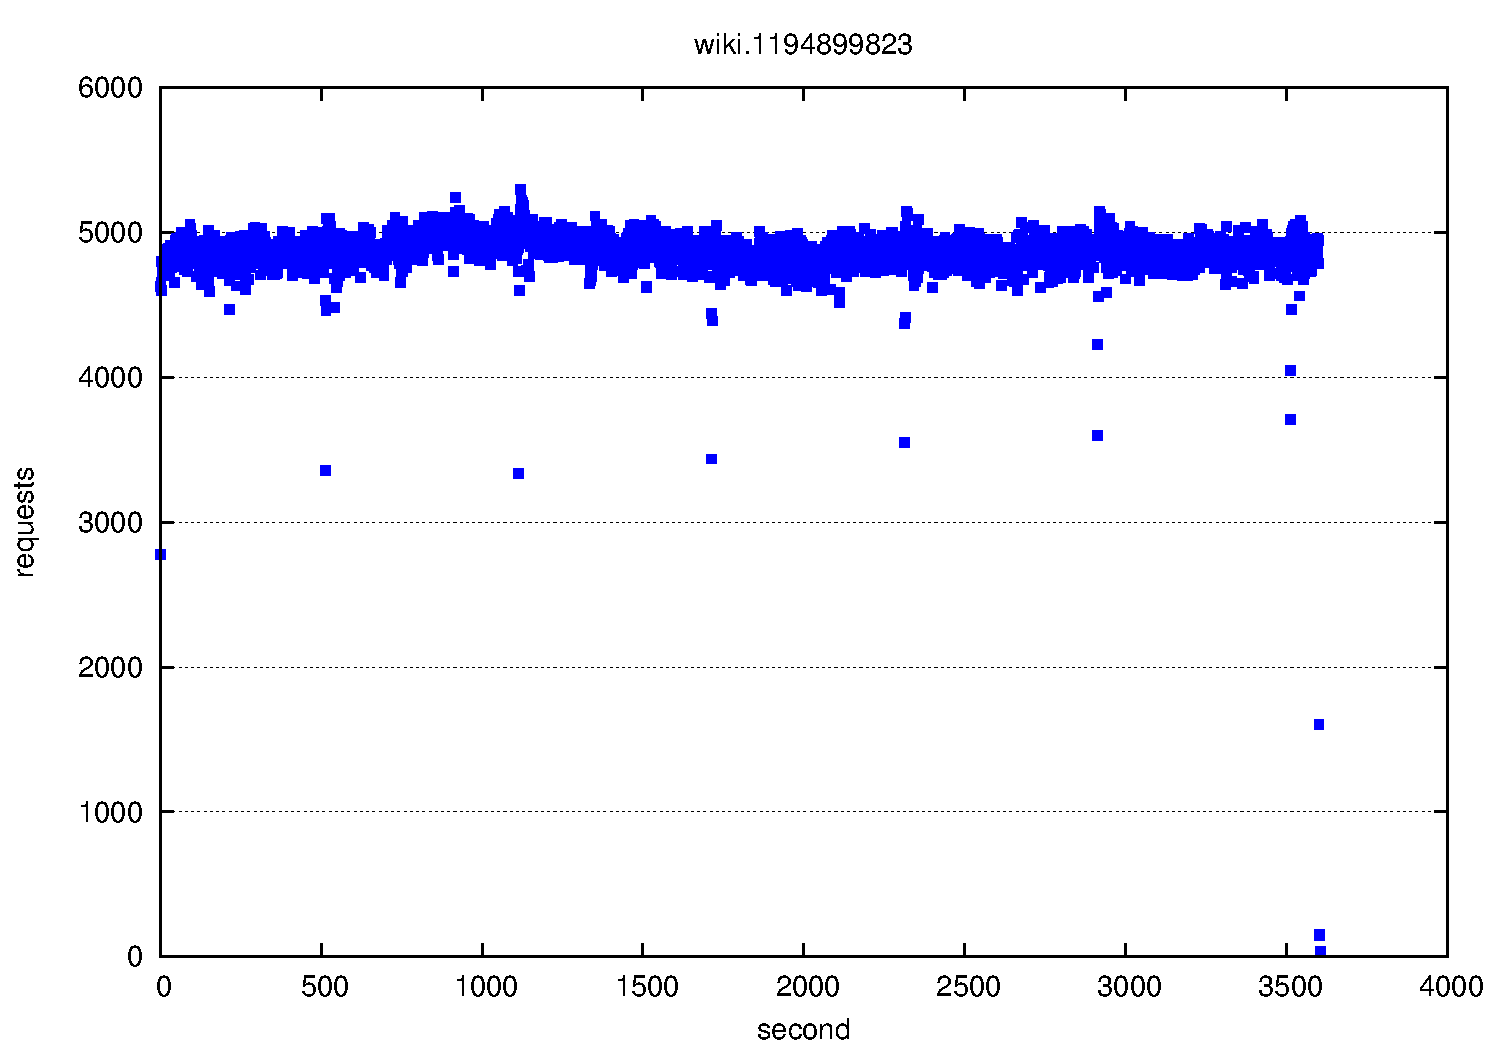
\includegraphics[width=\textwidth]{images/trace-full}
  \caption{Requests pro Sekunde der Datei \texttt{wiki.1194899823.gz}}
  \label{fig:trace-full}
\end{figure}

\begin{table}
  \centering
  \begin{tabular}{|rr|}\hline
    \textbf{General} & \\\hline
    tracefile: & wiki.1194899823.1194892290-1194894090.gz\\
    start time: & Mon, 12 Nov 2007 18:31:30 +0000\\
    end time: & Mon, 12 Nov 2007 19:01:30 +0000\\
    duration: & 1800.788 sec\\
    lines: & 4795845\\
    requests: & 4.795.845\\
    page requests: & 1.599.427 (33,3\%) \\
    media requests: & 3.196.418 (66,6\%) \\
    errors: & 0\\\hline\hline
    \textbf{Hosts} & \\\hline
    upload.wikimedia.org: & 3.196.418 (66,6\%) \\
    en.wikipedia.org: & 1.599.427 (33,3\%) \\\hline
  \end{tabular}
  \caption{Trace-Analyse der Datei \texttt{wiki.1194892290-1194894090.1194899823.gz}}
  \label{tab:trace-filtered}
\end{table}

\begin{figure}
  \centering
  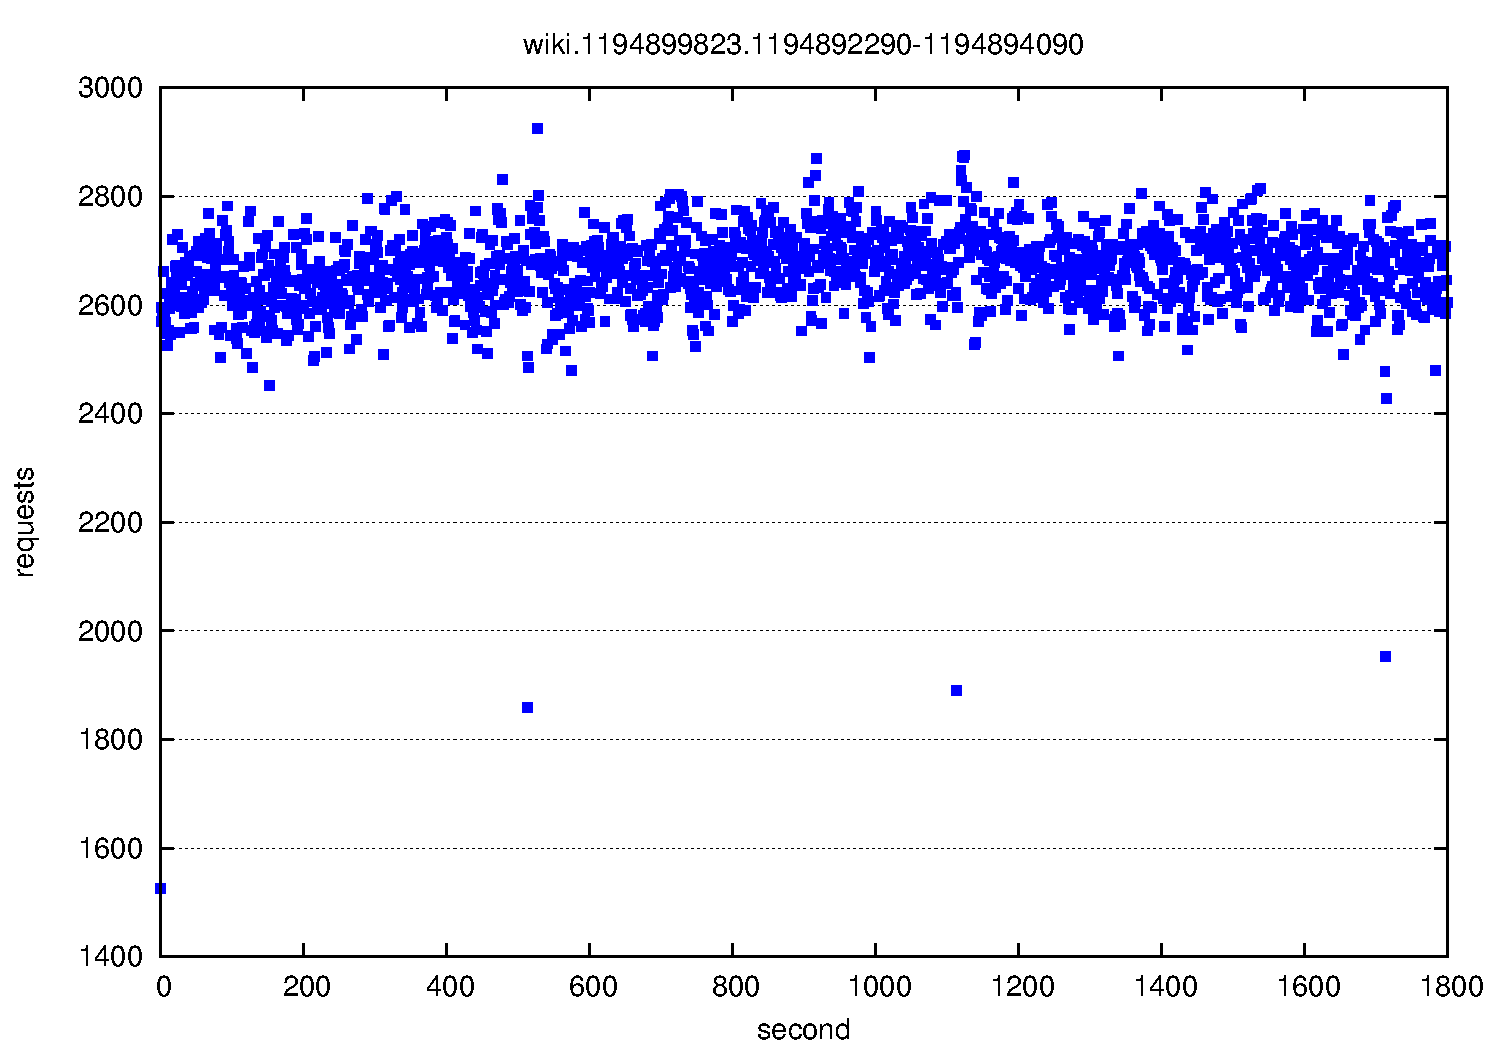
\includegraphics[width=\textwidth]{images/trace-filtered}
  \caption{Requests pro Sekunde der Datei \texttt{wiki.1194892290-1194894090.1194899823.gz}}
  \label{fig:trace-filtered}
\end{figure}

%%% Local Variables: 
%%% mode: latex
%%% TeX-master: "../master"
%%% End: 

% LocalWords:  Konfigurations httpd PHP MySQL ImageMagick Thumbnails gnuplot py
% LocalWords:  Mediawiki Dump xml sql mysqlimport Traces tar gzip bzip php SVN
% LocalWords:  LocalSettings Extensions extensions Repository Mediwiki index gz
% LocalWords:  Short RedHat gnome vfs SVG setup env ppr Sourcecode GIT Process
% LocalWords:  Klassendiagramm multiprocessing Pipes Logger SyncClient Pipe bzw
% LocalWords:  FileReader PipeReader FileWriter TraceAnalyser WikiAnalyser plot
% LocalWords:  TraceFilter WikiFilter HTTPAsyncClient FileClient asynchat trace
% LocalWords:  Requests Response HTTPCrawler FileCrawler asyncore Request async
% LocalWords:  FileCollector general filter Zeitstempel Wiedereinspielen clean
% LocalWords:  download images mysql archive output install String Usernamen rr
% LocalWords:  Thumbnail File Collector MediaWiki scp server ssh Host save time
% LocalWords:  tracefile start Mon Nov
